\chapter{Project}

This section will discuss the entities and requirements evaluated from the proposal.
\todo{e o design geral do project, overview das seccoes}

\section{Requirements}
Given the written proposal and eventual consultations with stakeholders, the general behavior and requirements of this application were evaluated. In regards to use cases, two actors were identified, a User that represents professors and employees that belongs to \gls{IPB} and a Administrator whose use-cases include classic \gls{CRUD} operations.

As an authenticated User, there are two goals that are covered by the use-case diagram shown in Figure~\ref{fig:userusecase}, Run a Query and Export a Spreadsheet. The former models the action of temporarily accessing some of the institution's information and the latter, even though taking the same steps, provides the user with a file that can be processed by other tools or used at a later time.

An authenticated Administrator, because he is expected to manage the system, is provided of more use-cases that follow a similar pattern, that is, managing the entities that compose the system by the means of \gls{CRUD} operations. Added to this, the use-case diagram found in Figure~\ref{fig:adminusecases} brings to light even another action, to ``Associate User and Permission'' that indicates the process of enabling an User to run a Query.

The proposal expresses the following requirements:
\begin{enumerate}
\item The system should be able to run queries in the database currently employed at the institution.\label{req:multidb}
\item Users can only run queries in which they have Permission to.\label{req:permission}
\item Query commands may be longer than 30 lines long.\label{req:longquery}
\item Running a Query yields a table that can be downloaded.\label{req:download}
\item No \gls{SQL} knowledge is needed to execute a Query.\label{req:noknowledge}
\item The system enables the insertion of new Queries.\label{req:addquery}
\end{enumerate}

\begin{figure}[h]
  \centering
  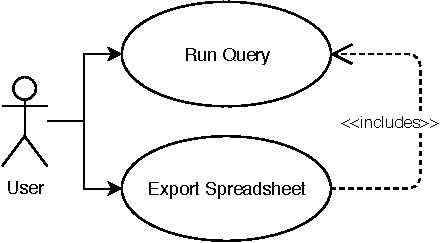
\includegraphics[width=.5\textwidth]{images/diagramas/userusecase}
  \caption{User use-case}\label{fig:userusecase}
\end{figure}

\begin{figure}[h]
  \centering
  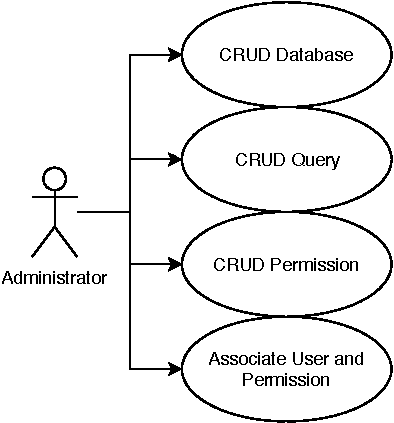
\includegraphics[width=.5\textwidth]{images/diagramas/adminusecase}
  \caption{Administrator use-cases}\label{fig:adminusecases}
\end{figure}

\begin{description}
\item[Database] Where a Query is run.\\
  It is responsible to hold the information that enables the access to a given database, effectively meeting requirement~\ref{req:multidb}.
  In the most basic form, a connection requires the network address and authentication credentials.
\item[User] Represents the person currently logged-in.\\
  It has two purposes, first is to differentiate users according to their roles, either ``Administrators'' or ``User'' so that certain actions are disabled, for example the Administrative task stated in requirement~\ref{req:addquery}
  The second is to be used when filtering Queries so that requirement~\ref{req:permission}
\item[Query] A script that is run in a Database and gather information into a single table.\\
  A \gls{SQL} script must be issued during a session with a Database.
  To fulfill requirement~\ref{req:noknowledge}, some meta information such as a title and a description so that the target audience is able to find the Query that fulfill their needs.
\item[Permission] The binding between Users and Queries.\\
  In order to fulfill requirement~\ref{req:permission}, this entity is responsible to handle the relation between a User and all the Queries that they may access.
\end{description}

\todo{Comentar a imaem}

\begin{figure}
  \centering
  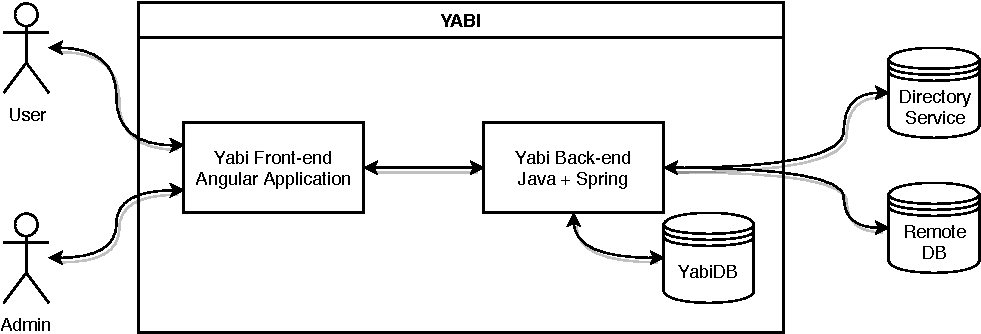
\includegraphics[width=\textwidth]{images/diagramas/overview.pdf}
  \caption{Yabi Overview}\label{fig:overview}
\end{figure}

\section{Project Details}
\todo{importante mas nao sei onde por ainda}
Queries must be associated to one Permission.
Users may have more than one permission.
The system must authenticate using the institute's centralized directory server.
An Administrator can manage the system by altering everything that is in the scope of this system.

Permissions is a central piece of this system. It's what associates users with information.
Permissions follow a hierarchy. There is a root Permission whose path is simply ``/'' and it's parent is itself.
There are two roles that any given user may be assigned to, either Administrator or User.

\section{Class Diagram}\label{tities}
\todo{citar a batida de nomes}
\todo{de alguma forma, chegou nesse diagrama}
\begin{figure}
  \centering
  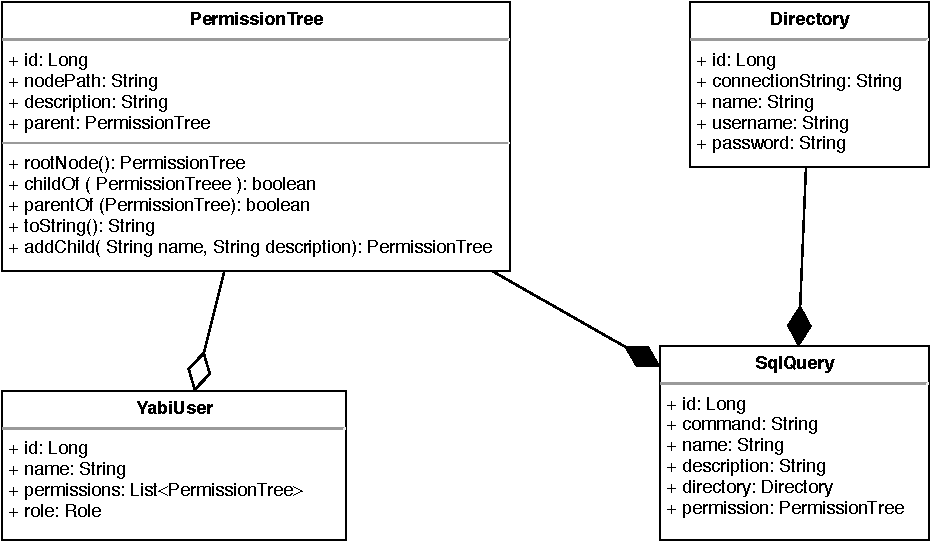
\includegraphics[width=.9\textwidth]{images/diagramas/class}
  \caption{Class diagram}\label{fig:classdiagram}
\end{figure}

\subsection{Query}
\dots
\subsection{Database}
\dots
\subsection{Query}\label{model:query}
\dots
\subsection{Permission}
\todo{O no raiz deve sempre existir, as permissoes sao pendiradas na arvore e a raiz precise ser boostrapped no deploy. se a raiz for deletada, nao tem como adicionar mais permissoes.}
\dots
\subsection{User}\label{model:user}
\dots

\section{Authentication and Authorization}\label{proj:auth}
\dots

\section{Template Sb-Admin-Material}
\dots
\section{Multi-Database Support}

\todo{Deve citar os bancos mais usados, e o banco mais usado pelo IPB (oracle)}

Even though the context in which the application described in this document will be primarily accessing Oracle databases, support for other databases was added to broaden its usefulness.

As far as the project for implementing this feature goes, Figure\ref{fig:multidbproj} hopefully describes the process. When a request to run a given Query arrives,
